\documentclass{beamer}
\usepackage{physics}
\usepackage{amsmath}
\usepackage{tikz}
\usepackage{mathdots}
\usepackage{yhmath}
\usepackage{cancel}
\usepackage{color}
\usepackage{siunitx}
\usepackage{array}
\usepackage{multirow}
\usepackage{amssymb}
\usepackage{gensymb}
\usepackage{tabularx}
\usepackage{extarrows}
\usepackage{booktabs}
\usetikzlibrary{fadings}
\usetikzlibrary{patterns}
\usetikzlibrary{shadows.blur}
\usetikzlibrary{shapes}
\usepackage{hyperref}

%Information to be included in the title page:
\title{Numerical bootstrap}
\author{Jinyuan Wu}
\institute{Department of Physics, Fudan University}
\date{2021}

\usetheme{Madrid}

\newcommand{\concept}[1]{\textbf{#1}}

\begin{document}

\frame{\titlepage}

\begin{frame}
\frametitle{Introduction}

\textbf{What's bootstrap}

\begin{itemize}
    \item A quantum theory = expectations of all Hermitian operators; 
    Hamiltonian/Lagrangian $\Leftrightarrow$ ``probability distribution''
    \item Constraint on the system $\Rightarrow$ relation between different $\expval{O}$'s (``\concept{data}'');
    independent $\expval{O}$'s $\Leftrightarrow$ parameters in the model
    \item Inequality constraint (e.g. positivity of $\expval{O^\dagger O}$) $\Rightarrow$ allowed 
    range of $\expval{O}$'s
    \item Solving a class of problems without mentioning explicitly the wave function/path integral: 
    hence the name \emph{bootstrap}
\end{itemize}

\vspace{1em}

\textbf{Why we need it}

\begin{itemize}
    \item Because it doesn't fail with strong non-perturbative effects. \footnote{\href{https://arxiv.org/abs/2108.11416}{arXiv 2108.11416}}
\end{itemize}

\end{frame}

\begin{frame}
\frametitle{Example: conformal bootstrap}

\begin{itemize}
    \item The most famous example: \concept{conformal bootstrap}
    \item Constraints: (spinless) two-point function 
    \begin{equation}
        \expval*{\mathcal{O}(x) \mathcal{O}(y)} = \frac{1}{\abs*{x - y}^{2 \Delta_\mathcal{O}}},
    \end{equation}
    three-point function 
    \begin{equation}
        \begin{aligned}
            &\quad \langle\mathcal{A}(x) \mathcal{B}(y) \mathcal{C}(z)\rangle \\
            &= \frac{f_{\mathcal{A B C}}}{|x-y|^{\Delta \mathcal{A}+\Delta_{\mathcal{B}}-\Delta_{\mathcal{C}}}|y-z|^{\Delta_{\mathcal{B}}+\Delta_{\mathcal{C}}-\Delta \mathcal{A}}|z-x|^{\Delta_{\mathcal{C}}+\Delta_{\mathcal{A}}-\Delta_{\mathcal{B}}}}
        \end{aligned}
    \end{equation}
    Higher order correlation functions: OPEs. 
    \item Independent parameters: $\{\Delta_{\mathcal{O}}, l_{\mathcal{O}}, f_{\mathcal{A} \mathcal{B} \mathcal{C}}\}$
    \item Inequality constraints (self-consistent conditions): determining the range of parameters
\end{itemize}

\end{frame}

\begin{frame}
\frametitle{Example: conformal bootstrap}

\begin{itemize}
    \item Example of conformal bootstrap: verify whether the critical point of 3D Ising model 
    is a CFT and its position in the allowed region \footnote{arXiv \href{https://arxiv.org/abs/1203.6064}{1203.6064}}
    \item Physical picture tells us there are two degrees of freedom: energy density $\epsilon$, spin field $\sigma$
    \item Below is Fig.~3 in the paper: comparing critical exponents of 3D Ising model, and the allowed range from conformal bootstrap
\end{itemize}

\begin{center}
    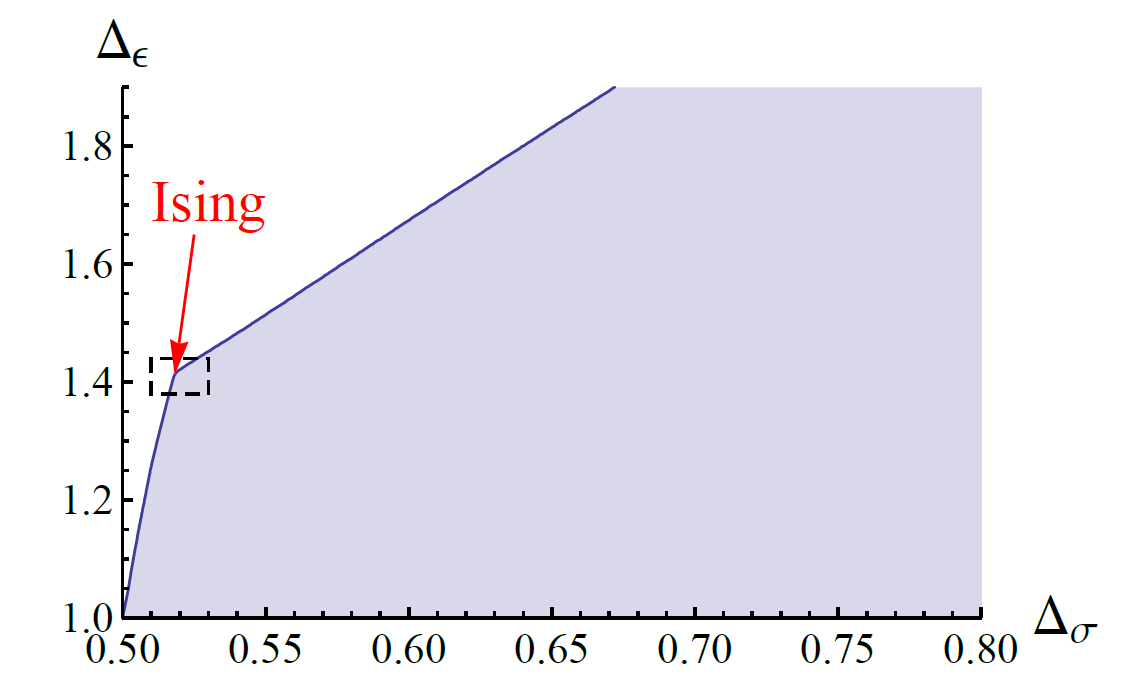
\includegraphics[width=0.5\textwidth]{3d-ising-cft-bootstrap-range.PNG}
\end{center}

\end{frame}

\begin{frame}
\frametitle{Bootstrap for generic systems}

\textbf{How to perform bootstrap for a generic system?}    

\begin{itemize}
    \item Correlation functions cannot be determined by countably infinite parameters: 
    no $\{\Delta_{\mathcal{O}}, l_{\mathcal{O}}, f_{\mathcal{A} \mathcal{B} \mathcal{C}}\}$.
    
    \textbf{Solution} Store $\expval{O_1(x_1) O_2(x_2) \cdots O_n (x_n)}$ separately. Symmetries reduce the size 
    of data: Suppose $C$ is a symmetry, 
    \begin{equation}
        \expval{OC} = \expval{CO}.
    \end{equation}
    Derivation similar to below.
    
    \item Hard to get OPE
    
    \textbf{Solution} Suppose we are working on a state whose density matrix is determined solely by $H$,
    then we have 
    \begin{equation}
        \expval*{O H} = \trace (\rho(H) O H) = \trace(H \rho(H) O) = \trace(\rho(H) H O)  = \expval*{H {O}}
    \end{equation}
    for all operators $O$. If we are working on energy eigenstates (i.e with definite $E$), we have 
    \begin{equation}
        \expval{O H} = E \expval{O}, \quad E = \expval{H}.
    \end{equation}
\end{itemize}

\end{frame}

\begin{frame}
\frametitle{Bootstrap for generic systems}

\begin{itemize}
    \item The equality constraints used together with the positivity constraint 
    \begin{equation}
        \expval*{O^\dagger O} \geq 0
    \end{equation}
    for every $O$ defines an allowed region - the feasible domain for the following optimization.
    \item To get ground state information, minimize $\expval*{H}$ globally.
    \item To get information about excited states, find local minima of $\expval*{H}$.
\end{itemize} 

\begin{center}
    

\tikzset{every picture/.style={line width=0.75pt}} %set default line width to 0.75pt        

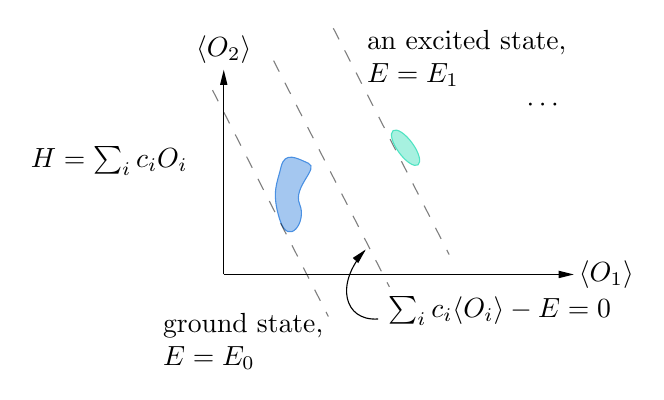
\begin{tikzpicture}[x=0.75pt,y=0.75pt,yscale=-0.6,xscale=0.6]
%uncomment if require: \path (0,353); %set diagram left start at 0, and has height of 353

%Straight Lines [id:da904255078328454] 
\draw    (177,246) -- (456,246) ;
\draw [shift={(458,246)}, rotate = 180] [fill={rgb, 255:red, 0; green, 0; blue, 0 }  ][line width=0.08]  [draw opacity=0] (12,-3) -- (0,0) -- (12,3) -- cycle    ;
%Straight Lines [id:da28860077544833507] 
\draw    (177,246) -- (177,83.73) ;
\draw [shift={(177,81.73)}, rotate = 90] [fill={rgb, 255:red, 0; green, 0; blue, 0 }  ][line width=0.08]  [draw opacity=0] (12,-3) -- (0,0) -- (12,3) -- cycle    ;
%Shape: Polygon Curved [id:ds05129166801576668] 
\draw  [color={rgb, 255:red, 74; green, 144; blue, 226 }  ,draw opacity=1 ][fill={rgb, 255:red, 74; green, 144; blue, 226 }  ,fill opacity=0.5 ] (223,159.73) .. controls (226,146.73) and (236,152.73) .. (245,156.73) .. controls (254,160.73) and (232,175.73) .. (238,189.73) .. controls (244,203.73) and (229,224.27) .. (222,202) .. controls (215,179.73) and (220,172.73) .. (223,159.73) -- cycle ;
%Straight Lines [id:da6483527344854445] 
\draw [color={rgb, 255:red, 0; green, 0; blue, 0 }  ,draw opacity=0.5 ] [dash pattern={on 4.5pt off 4.5pt}]  (168,98) -- (261,279.73) ;
%Straight Lines [id:da0036541181567224523] 
\draw [color={rgb, 255:red, 0; green, 0; blue, 0 }  ,draw opacity=0.5 ] [dash pattern={on 4.5pt off 4.5pt}]  (217,74.27) -- (310,256) ;
%Straight Lines [id:da34767057063343554] 
\draw [color={rgb, 255:red, 0; green, 0; blue, 0 }  ,draw opacity=0.5 ] [dash pattern={on 4.5pt off 4.5pt}]  (265,48.27) -- (358,230) ;
%Shape: Ellipse [id:dp302165402812995] 
\draw  [color={rgb, 255:red, 80; green, 227; blue, 194 }  ,draw opacity=1 ][fill={rgb, 255:red, 80; green, 227; blue, 194 }  ,fill opacity=0.5 ] (312.97,130.5) .. controls (310.07,132.62) and (312.21,140.48) .. (317.75,148.06) .. controls (323.29,155.64) and (330.13,160.08) .. (333.03,157.96) .. controls (335.93,155.84) and (333.79,147.98) .. (328.25,140.4) .. controls (322.71,132.81) and (315.87,128.38) .. (312.97,130.5) -- cycle ;
%Curve Lines [id:da7414078371933952] 
\draw    (301,281.73) .. controls (273.42,283.7) and (266.21,253.65) .. (289.9,227.21) ;
\draw [shift={(291,226)}, rotate = 133.09] [fill={rgb, 255:red, 0; green, 0; blue, 0 }  ][line width=0.08]  [draw opacity=0] (12,-3) -- (0,0) -- (12,3) -- cycle    ;

% Text Node
\draw (460,246) node [anchor=west] [inner sep=0.75pt]    {$\langle O_{1} \rangle $};
% Text Node
\draw (177,78.33) node [anchor=south] [inner sep=0.75pt]    {$\langle O_{2} \rangle $};
% Text Node
\draw (307,261.4) node [anchor=north west][inner sep=0.75pt]    {$\sum _{i} c_{i} \langle O_{i} \rangle -E=0$};
% Text Node
\draw (259,275) node [anchor=north east] [inner sep=0.75pt]   [align=left] {ground state,\\$\displaystyle E=E_{0}$};
% Text Node
\draw (290,97.27) node [anchor=south west] [inner sep=0.75pt]   [align=left] {an excited state,\\$\displaystyle E=E_{1}$};
% Text Node
\draw (418,103.4) node [anchor=north west][inner sep=0.75pt]    {$\cdots $};
% Text Node
\draw (20,141.4) node [anchor=north west][inner sep=0.75pt]    {$H=\sum _{i} c_{i} O_{i}$};


\end{tikzpicture}

\end{center}

\end{frame}

\begin{frame}
\frametitle{Bootstrap for generic systems}

\textbf{The procedure of numerical bootstrap}   

\begin{itemize}
    \item Determine a set of operators 
\end{itemize}

\end{frame}

\begin{frame}
\frametitle{Example: $x^4$ nonlinear oscillator}

\begin{equation}
    H = x^2 + p^2 + g x^4.
\end{equation}

\begin{itemize}
    \item Symmetry: $x \to -x$ $\Rightarrow$ $\expval*{x^n} = 0$ with odd $n$
    \item 
\end{itemize}

\end{frame}

\end{document}